\documentclass{beamer}

\usepackage[utf8x]{inputenc}
\usepackage{graphicx}
\usepackage{amsthm,amssymb,amsbsy,amsmath,amsfonts,amssymb,amscd}
\usepackage{dsfont}
\usepackage{array}
\newcolumntype{N}{@{}m{2pt}@{}}
\usepackage{tikz}
%\usetikzlibrary{arrows}
%\tikzstyle{block}=[draw opacity=0.7,line width=1.4cm]

\useoutertheme[subsection=false]{miniframes}
\usepackage{lmodern}

\setbeamercolor{author in head/foot}{fg=gray,bg=white}
\setbeamercolor{title in head/foot}{fg=gray,bg=white}
\setbeamercolor{page number in head/foot}{fg=gray,bg=white}
\setbeamercolor{section in head/foot}{bg=black,fg=gray}
\setbeamercolor{subsection in head/foot}{bg=black,fg=gray}

%%%%%%%%%%%%%%%%%%%%%%%%
% GENERAL BEAMER STYLE :

\setbeamertemplate{footline}{
  \hbox{%
    \begin{beamercolorbox}[wd=.2\paperwidth,ht=2ex,dp=1ex,left]{author in head/foot}%
      \hskip1em\usebeamerfont{author in head/foot}\insertshortauthor
    \end{beamercolorbox}%
    \begin{beamercolorbox}[wd=.7\paperwidth,ht=2ex,dp=1ex,center]{title in head/foot}%
      \usebeamerfont{title in head/foot}\insertshorttitle
    \end{beamercolorbox}%
    \begin{beamercolorbox}[wd=.1\paperwidth,ht=2ex,dp=1ex,right]{page number in head/foot}%
      \usebeamerfont{page number in head/foot}\insertframenumber{} / \inserttotalframenumber
      \kern1em 
    \end{beamercolorbox}
  }
}

\setbeamercolor{alerted text}{fg=red!80!black}
\setbeamercolor{itemize/enumerate subbody}{fg=gray!70!black}
\setbeamertemplate{itemize item}[square]
\setbeamertemplate{itemize subitem}[triangle]%{{\textendash}}
\setbeamerfont{itemize/enumerate subbody}{size=\footnotesize}
\setbeamerfont{itemize/enumerate subitem}{size=\footnotesize}

\setbeamertemplate{navigation symbols}{}

\AtBeginSection{
\begin{frame}
    \begin{centering}
    \begin{beamercolorbox}[sep=12pt,center]{part title}
    \usebeamerfont{section title}\insertsection\par
    \end{beamercolorbox}
    \end{centering}
\end{frame}
}

 


\title[Majeure Data Science -- Surrogate models and GPR]{\texorpdfstring{ \small Surrogate models and Gaussian Process regression -- lecture 5/5 \\ \vspace{3mm} \LARGE Advanced GP models}{}}
\author[Mines St-\'Etienne ]{Mines St-\'Etienne -- Majeure Data Science -- 2016/2017}
\institute{\texorpdfstring{Nicolas Durrande (durrande@emse.fr)}{}}
\date{\null}

\DeclareMathOperator*{\Var}{var}
\DeclareMathOperator*{\E}{E}
\DeclareMathOperator*{\Cov}{cov}
\newcommand\PR[1]{\mathrm{P}\left(#1 \right)}
\newcommand\PS[1]{{\langle #1 \rangle}_\mathcal{H}}
\newcommand\PSi[2]{{ \left \langle #1 \right \rangle}_{\! #2}}
\newcommand\N[2]{{|| #1 ||}_{\! #2}}
\newcommand\dx{\, \mathrm{d}}
\newcommand\textequal{\rule[.4ex]{4pt}{0.4pt}\llap{\rule[.7ex]{4pt}{0.4pt}}}
\newcommand{\argmin}{\operatornamewithlimits{argmin}}
\makeatletter
\newcommand{\shorteq}{%
  \settowidth{\@tempdima}{a}% Width of hyphen
  \resizebox{\@tempdima}{\height}{=}%
}
\makeatother

\newenvironment{psmallmatrix}
  {\left(\begin{smallmatrix}}
  {\end{smallmatrix}\right)}


%%%%%%%%%%%%%%%%%%%%%%%%%%%%%%%%%%%%%%%%%%%%%%%%%%%%%%
%%%%%%%%%%%%%%%%%%%%%%%%%%%%%%%%%%%%%%%%%%%%%%%%%%%%%%
%%%%%%%%%%%%%%%%%%%%%%%%%%%%%%%%%%%%%%%%%%%%%%%%%%%%%%
\begin{document}
\setbeamercolor{author in head/foot}{fg=gray,bg=white}
\setbeamercolor{title in head/foot}{fg=gray,bg=white}
\setbeamercolor{page number in head/foot}{fg=gray,bg=white}
\setbeamercolor{section in head/foot}{bg=black,fg=gray}
\setbeamercolor{subsection in head/foot}{bg=black,fg=gray}

%%%%%%%%%%%%%%%%%%%%%%%%%%%%%%%%%%%%%%%%%%%%%%%%%%%%%%
\begin{frame}
  \titlepage
\end{frame}

%%%%%%%%%%%%%%%%%%%%%%%%%%%%%%%%%%%%%%%%%%%%%%%%%%%%%%
%%%%%%%%%%%%%%%%%%%%%%%%%%%%%%%%%%%%%%%%%%%%%%%%%%%%%%
\section[Multioutputs GPR]{Multioutputs GPR / GPR with categorical inputs}
\subsection{}

%%%%%%%%%%%%%%%%%%%%%%%%%%%%%%%%%%%%%%%%%%%%%%%%%%%%%%
\begin{frame}{}
\begin{exampleblock}{Example}
	We observe the temperature in two cities $A$ and $B$ for a few time points $X_A$ and $X_B$. We assume a Gaussian process prior for these $T_A(t)$ and $T_B(t)$. What would be your prediction for the temperature in $A$ at a new time point $t$?
\end{exampleblock}
\pause
Ideally, we are interested in $T_A(t)|T_A(X_A), T_B(X_B)$. If $(T_A(t),\ T_A(X_A),\ T_B(X_B))$ is a Gaussian vector, we know how to compute the conditional distribution. However, it requires the cross covariance $k_{AB}(t,t') = \Cov[T_A(t),T_B(t')]$.
\end{frame}

%%%%%%%%%%%%%%%%%%%%%%%%%%%%%%%%%%%%%%%%%%%%%%%%%%%%%%
\begin{frame}{}
\begin{exampleblock}{Exercise}
Compute the distribution of $T_A(t)|T_A(X_A), T_B(X_B)$.
\end{exampleblock}
\pause
\begin{exampleblock}{Solution}
\vspace{2mm}
The conditional mean is:
\small
\begin{equation*}
	\begin{split}
		m_A(t) &= \E[T_A(t)|T_A(X_A) \shorteq F_A, T_B(X_B) \shorteq F_B] \\
		& \begin{pmatrix}
			k_A(t,X_A) & k_{AB}(t,X_B)
		\end{pmatrix}
		\begin{pmatrix}
			k_A(X_A,X_A) & k_{AB}(X_A,X_B) \\
			k_{AB}(X_A,X_B)^t & k_{B}(X_B,X_B) \\
		\end{pmatrix}^{-1}
		\begin{pmatrix}
			F_A \\
			F_B \\
		\end{pmatrix}
	\end{split}
\end{equation*}
\normalsize
The conditional covariance is:
\small
\begin{equation*}
	\begin{split}
		c_A(t,t') &=  \Cov[T_A(t),T_A(t')|T_A(X_A) \shorteq F_A, T_B(X_B) \shorteq F_B] \\
		&= k_A(t,t') - 
		\begin{pmatrix}
			k_A(t,X_A) & k_{AB}(t,X_B)
		\end{pmatrix} \\
		&  \hspace{2.5cm} \times
		\begin{pmatrix}
			k_A(X_A,X_A) & k_{AB}(X_A,X_B) \\
			k_{AB}(X_A,X_B)^t & k_{B}(X_B,X_B) \\
		\end{pmatrix}^{-1}
		\begin{pmatrix}
			k_A(t',X_A)^t \\
			k_{AB}(t',X_B)^t
		\end{pmatrix}
	\end{split}
	%\label{eq:multiGPR}
\end{equation*}
\end{exampleblock}
\end{frame}

%%%%%%%%%%%%%%%%%%%%%%%%%%%%%%%%%%%%%%%%%%%%%%%%%%%%%%
\begin{frame}{}
\begin{example}
	If we do the same thing fot $T_B$ we obtain:
	\begin{center}
	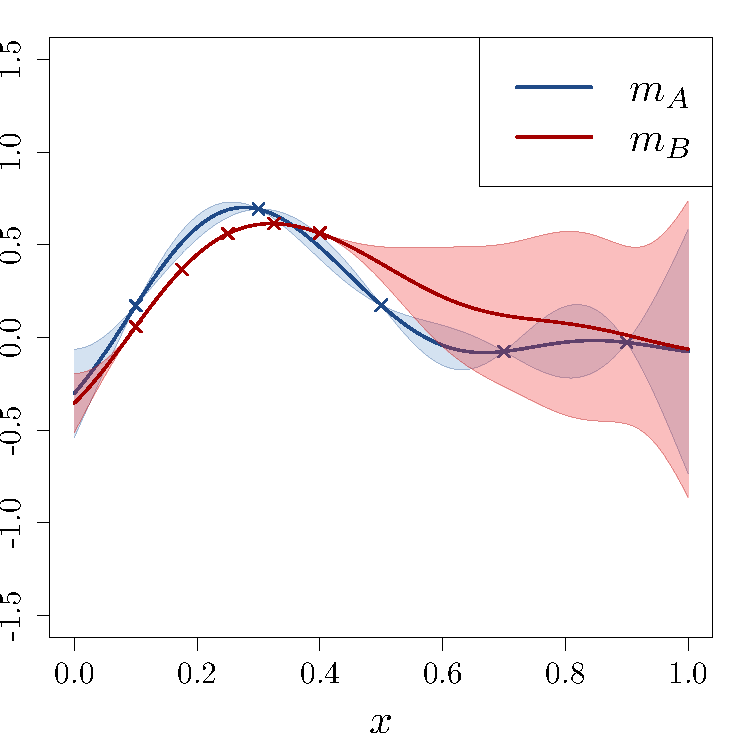
\includegraphics[height=7cm]{figures/R/ch2_multiGPR1}
	\end{center}
\end{example}
\end{frame}

%%%%%%%%%%%%%%%%%%%%%%%%%%%%%%%%%%%%%%%%%%%%%%%%%%%%%%
\begin{frame}{}
Instead of considering the GP to be multioutput, it is possible to see the GP as having one input but one extra categorical variable:
\begin{equation*}
 Z(t,c) = 
 \begin{cases}
   Z_A(t) & \text{if } c=A	\\
   Z_B(t) & \text{if } c=B.	
 \end{cases}
\end{equation*}
\begin{exampleblock}{Exercise:}
	Compute the kernel of $Z$.
\end{exampleblock}
\pause
\vspace{3mm}
With this settings, the conditional mean
\small
\begin{equation*}
	\begin{split}
		m_A(t) &= 
		 \begin{pmatrix}
			k_A(t,X_A) & k_{AB}(t,X_B)
		\end{pmatrix}
		\begin{pmatrix}
			k_A(X_A,X_A) & k_{AB}(X_A,X_B) \\
			k_{AB}(X_A,X_B)^t & k_{B}(X_B,X_B) \\
		\end{pmatrix}^{-1}
		\begin{pmatrix}
			F_A \\
			F_B \\
		\end{pmatrix}
	\end{split}
\end{equation*}
\normalsize
writes as an usual conditional mean
\small
\begin{equation*}
	\begin{split}
		m_A(t) = m(t,A) = \E[T(t,A)|T(X) \shorteq F] = 
		k(\begin{psmallmatrix} t \\ A \end{psmallmatrix},X) k(X,X)^{-1} F
	\end{split}
\end{equation*}
\normalsize
\end{frame}


%%%%%%%%%%%%%%%%%%%%%%%%%%%%%%%%%%%%%%%%%%%%%%%%%%%%%%
\begin{frame}{}
\begin{example}
	We obtain this representation for the model
	\begin{center}
	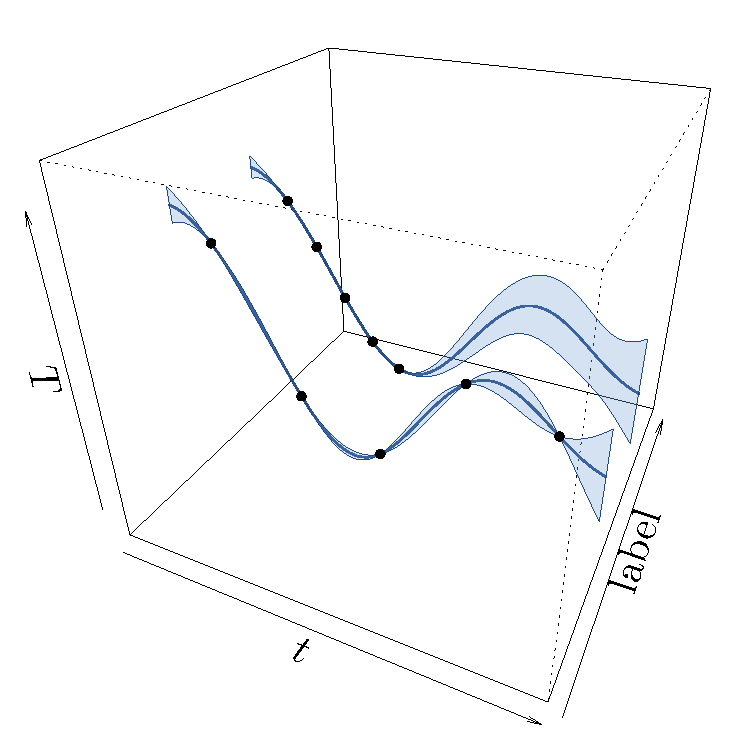
\includegraphics[height=7cm]{figures/R/ch2_multiGPR}
	\end{center}
\end{example}
\end{frame}


%%%%%%%%%%%%%%%%%%%%%%%%%%%%%%%%%%%%%%%%%%%%%%%%%%%%%%
\begin{frame}{}
In the end, multioutputs GPs can be seen as GPs with one extra categorical variable indicating the output label.\\
\vspace{5mm}
All the math stay the same, we just need to specify a covariance function that takes into account this extra variable. A common approach is to consider a product covariance structure
\begin{equation*}
k\left( \begin{psmallmatrix} \phantom{'}t\phantom{'} \\ \phantom{'}c\phantom{'} \end{psmallmatrix},\begin{psmallmatrix} t' \\ c' \end{psmallmatrix} \right) = k_{cont}(t,t') k_{disc}(c,c')
\end{equation*}
where $k_{disc}(c,c')$ can be described by a covariance matrix. In practice, this covariance matrix has to be estimated. 

\end{frame}

%%%%%%%%%%%%%%%%%%%%%%%%%%%%%%%%%%%%%%%%%%%%%%%%%%%%%%
\begin{frame}{}
If there are \textbf{2 outputs} (or 2 levels for the categorical variable), it is a $2 \times 2$ covariance matrix. It can be parameterised by
\small
$$k_{disc} = 
\begin{pmatrix}
	\sigma_1^2 & \sigma_1 \sigma_2 \rho \\
	\sigma_1 \sigma_2 \rho & \sigma_2^2 \\
\end{pmatrix}$$
\normalsize
with  $\sigma_1,\ \sigma_2 \geq 0$ and $\rho \in [-1,1]$. The latter can be estimated by ML.\\
\vspace{5mm}
\textbf{In higher dimension} (say $k$), it is possible to consider the following parameterization for $k_{disc}$:
\small
$$k_{disc} = W W^T$$
\normalsize
where $W$ is a $k \times l$ matrix. The choice of $l$ allows to tune the complexity of the estimation.

\end{frame}

%%%%%%%%%%%%%%%%%%%%%%%%%%%%%%%%%%%%%%%%%%%%%%%%%%%%%%
\begin{frame}{}
It is also possible to include in models observations more sophisticated than $Z(X)=F$... \\
\vspace{5mm}
For instance, if we know the integral of the function to approximate and it's derivative in a few points, we want to consider
$$ Z \ \left| \ Z(X) = F, \int Z = a, \frac{\dx Z}{\dx x}(X')= F' \right. $$
\end{frame}

%%%%%%%%%%%%%%%%%%%%%%%%%%%%%%%%%%%%%%%%%%%%%%%%%%%%%%
\begin{frame}{}
\begin{example}
	If we take into account that the function is centred, we obtain:
	\begin{center}
	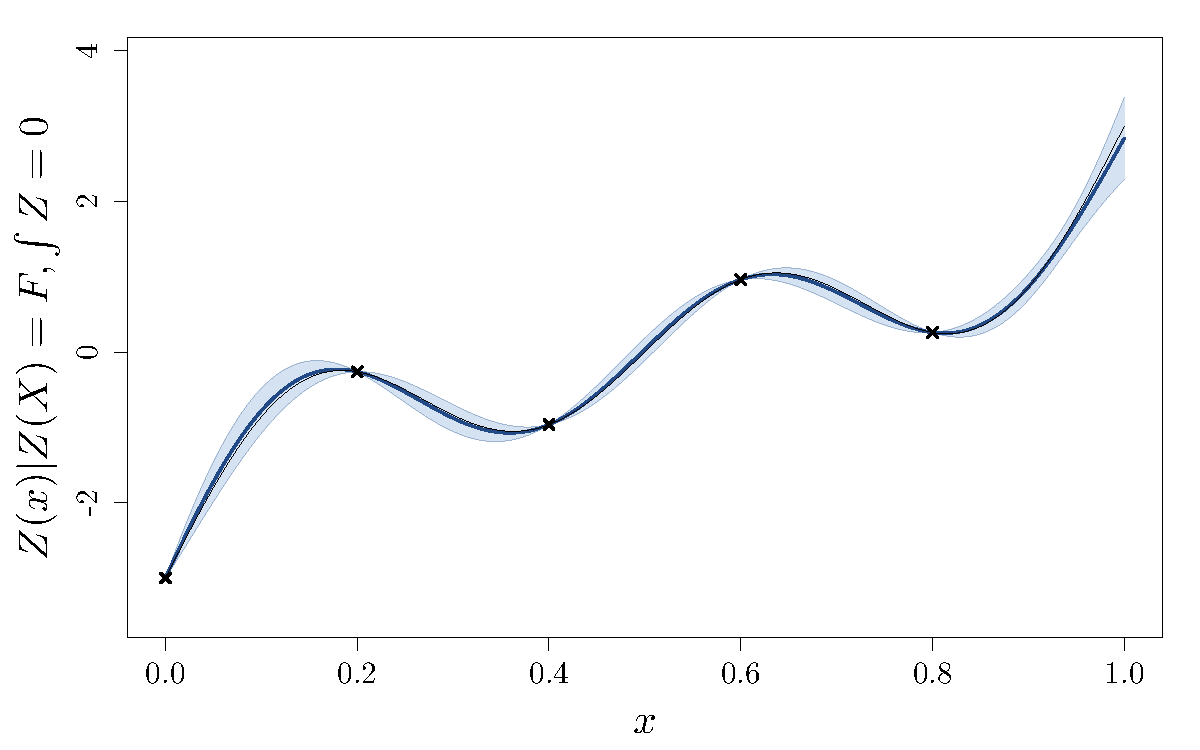
\includegraphics[height=6cm]{figures/R/exotic_int}
	\end{center}
\end{example}
\end{frame}

%%%%%%%%%%%%%%%%%%%%%%%%%%%%%%%%%%%%%%%%%%%%%%%%%%%%%%
\begin{frame}{}
\begin{example}
	Whereas if we ignore it:
	\begin{center}
	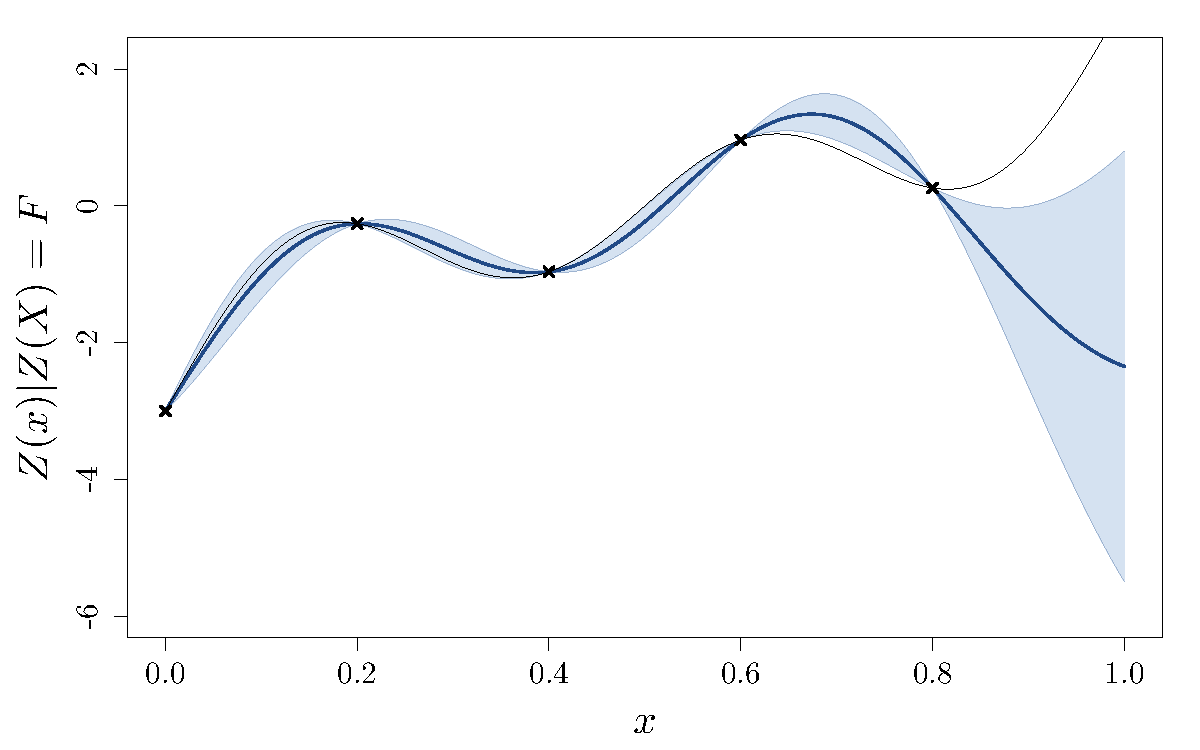
\includegraphics[height=6cm]{figures/R/exotic_pasint}
	\end{center}
\end{example}
\end{frame}

%%%%%%%%%%%%%%%%%%%%%%%%%%%%%%%%%%%%%%%%%%%%%%%%%%%%%%
\begin{frame}{}
Similarly, we can include in a model some derivative observations:
	\begin{center}
	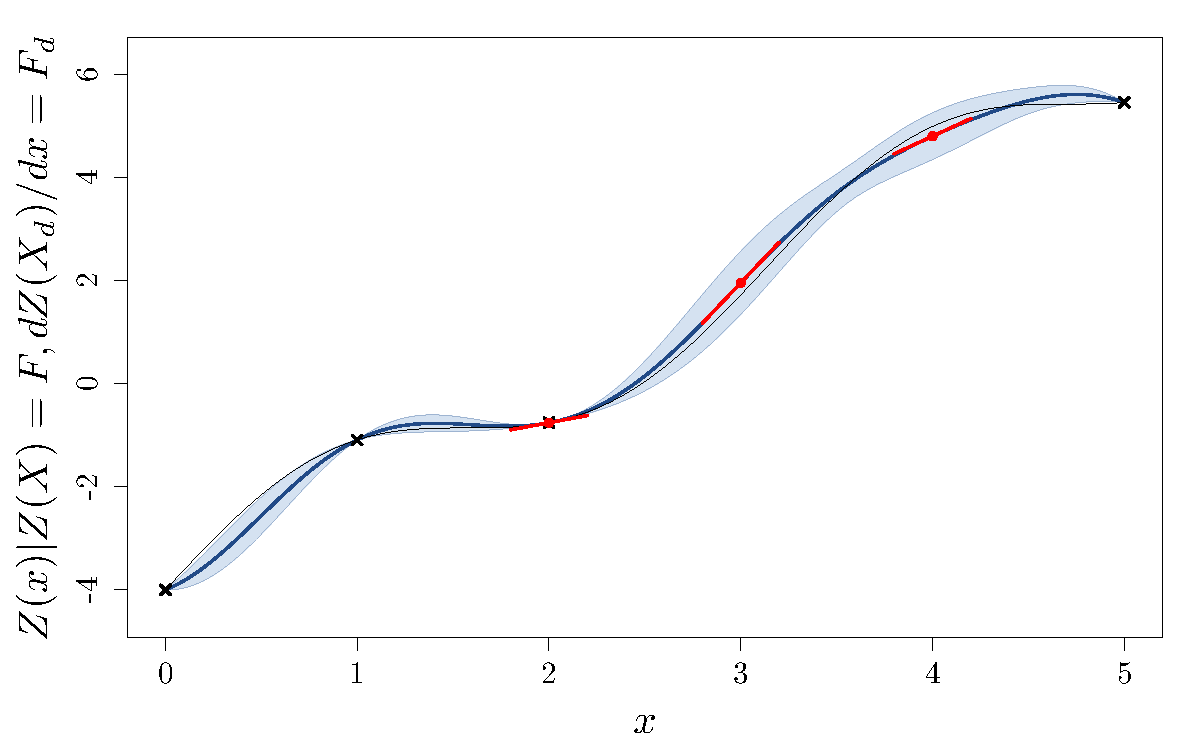
\includegraphics[height=6cm]{figures/R/exotic_der}
	\end{center}
\end{frame}

%%%%%%%%%%%%%%%%%%%%%%%%%%%%%%%%%%%%%%%%%%%%%%%%%%%%%%
\begin{frame}{}
We can see interesting behaviour if we look at a model with only derivatives.
	\begin{center}
	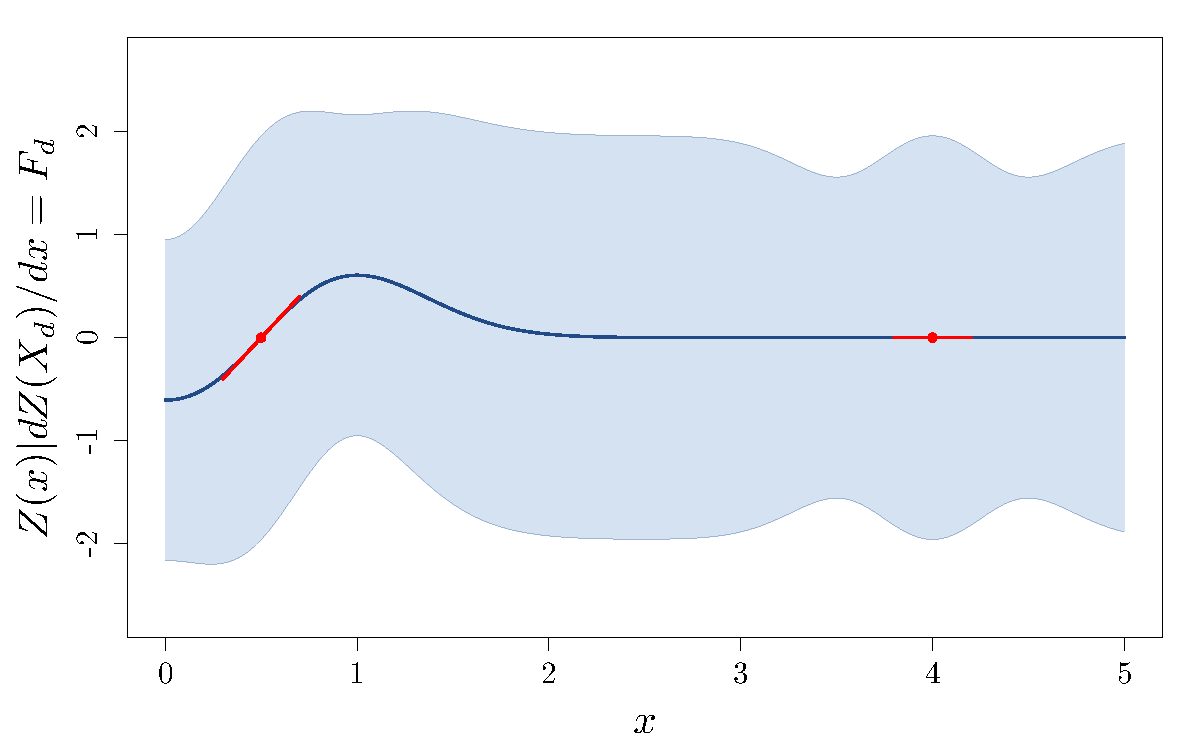
\includegraphics[height=6cm]{figures/R/exotic_deronly}
	\end{center}
\end{frame}

%%%%%%%%%%%%%%%%%%%%%%%%%%%%%%%%%%%%%%%%%%%%%%%%%%%%%%
\begin{frame}{}
As always, we can simulate conditional paths:
	\begin{center}
	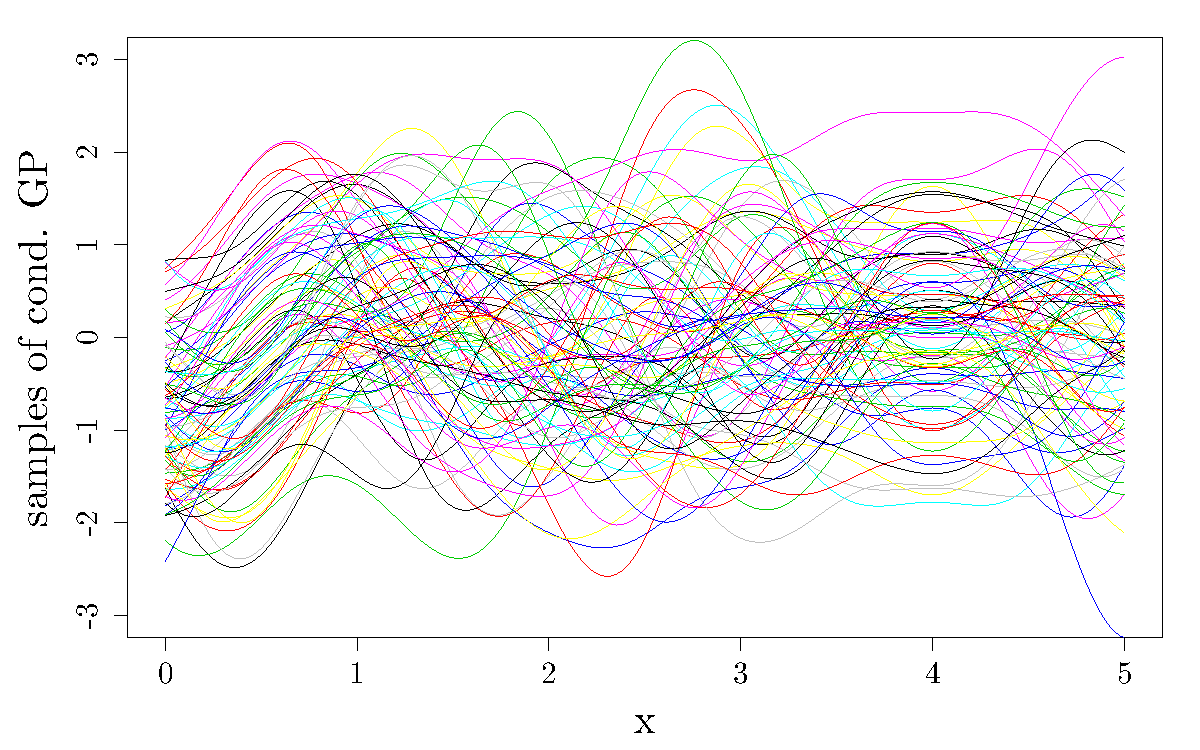
\includegraphics[height=6cm]{figures/R/exotic_simul}
	\end{center}
\end{frame}

%%%%%%%%%%%%%%%%%%%%%%%%%%%%%%%%%%%%%%%%%%%%%%%%%%%%%%%%%%%%%%%%%%%
%%%%%%%%%%%%%%%%%%%%%%%%%%%%%%%%%%%%%%%%%%%%%%%%%%%%%%%%%%%%%%%%%%%
\section[GPR Application]{Example of GPR application: Detecting periodicity in gene expression}
\subsection{}

%%%%%%%%%%%%%%%%%%%%%%%%%%%%%%%%%%%%%%%%%%%%%%%%%%%%%%
\begin{frame}{}
The 24 hour cycle of days can be observed in the oscillations of many physiological processes of living beings.\\
\begin{examples}
 Body temperature, jet lag, sleep, ... but also observed for plants, micro-organisms, etc.
\end{examples}
\vspace{0.5cm}
This phenomenon is called the \alert{circadian rhythm} and the mechanism driving this cycle is the \alert{circadian clock}. \\
\vspace{0.5cm}
To understand how the circadian clock operates at the gene level, biologist look at the temporal evolution of gene expression. 
\end{frame}


%%%%%%%%%%%%%%%%%%%%%%%%%%%%%%%%%%%%%%%%%%%%%%%%%%%%%%
\begin{frame}{}
\vspace{0.75cm}
The aim of gene expression is to measure the activity of various genes:
\begin{center}
 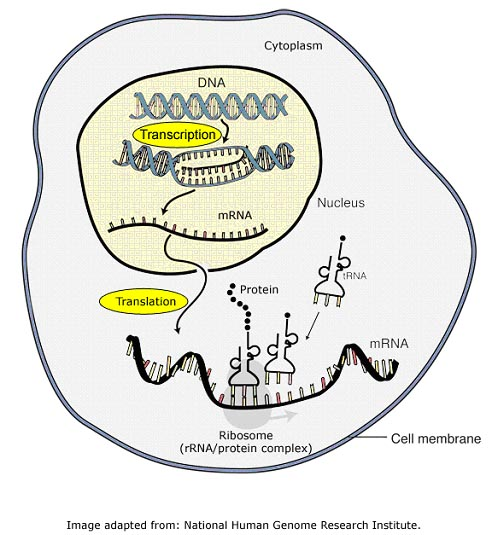
\includegraphics[height=6.5cm]{figures/DNAtranscription} 
\end{center}
\end{frame}

%%%%%%%%%%%%%%%%%%%%%%%%%%%%%%%%%%%%%%%%%%%%%%%%%%%%%%
\begin{frame}{}
\vspace{0.5cm}
The mRNA concentration is measured with microarray experiments\\
\vspace{0.25cm}
\begin{center}
 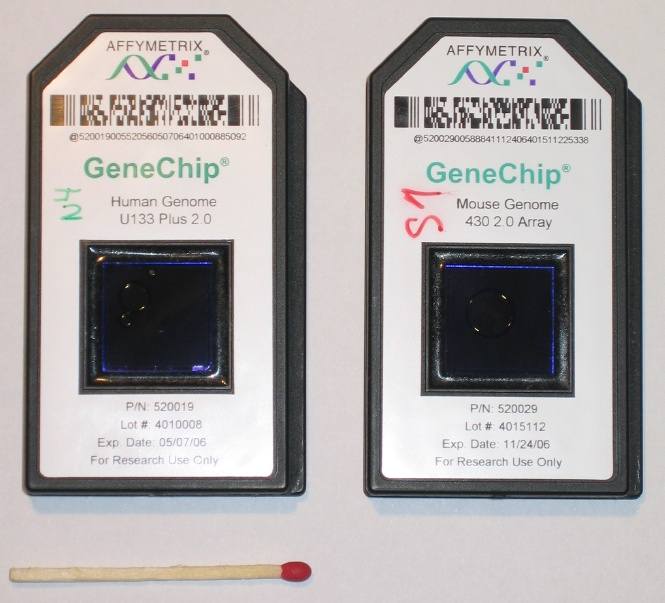
\includegraphics[height=3.8cm]{figures/Affymetrix} \qquad \qquad 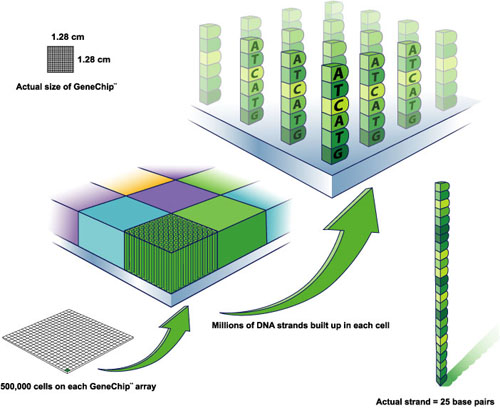
\includegraphics[height=3.8cm]{figures/microarray} 
\end{center}
\vspace{0.25cm}
The chip is then scanned to determine the occupation of each cell and reveal the concentration of mRNA. 
\end{frame}

%%%%%%%%%%%%%%%%%%%%%%%%%%%%%%%%%%%%%%%%%%%%%%%%%%%%%%
\begin{frame}{}
Experiments to study the circadian clock are typically:
\begin{enumerate}
 \item Expose the organism to a 12h light / 12h dark cycle
 \item at t=0, transfer to constant light
 \item perform a microarray experiment every 4 hours to measure gene expression
\end{enumerate}
 
\begin{block}{}
Regulators of the circadian clock are often rhythmically regulated.\\
\qquad \alert{$\Rightarrow$ identifying periodically expressed genes gives an insight on the overall mechanism.}
\end{block}
\end{frame}

%%%%%%%%%%%%%%%%%%%%%%%%%%%%%%%%%%%%%%%%%%%%%%%%%%%%%%
\begin{frame}{}
\begin{block}{}
In practice, we have for each gene:
\vspace{.3cm}
\begin{center}
 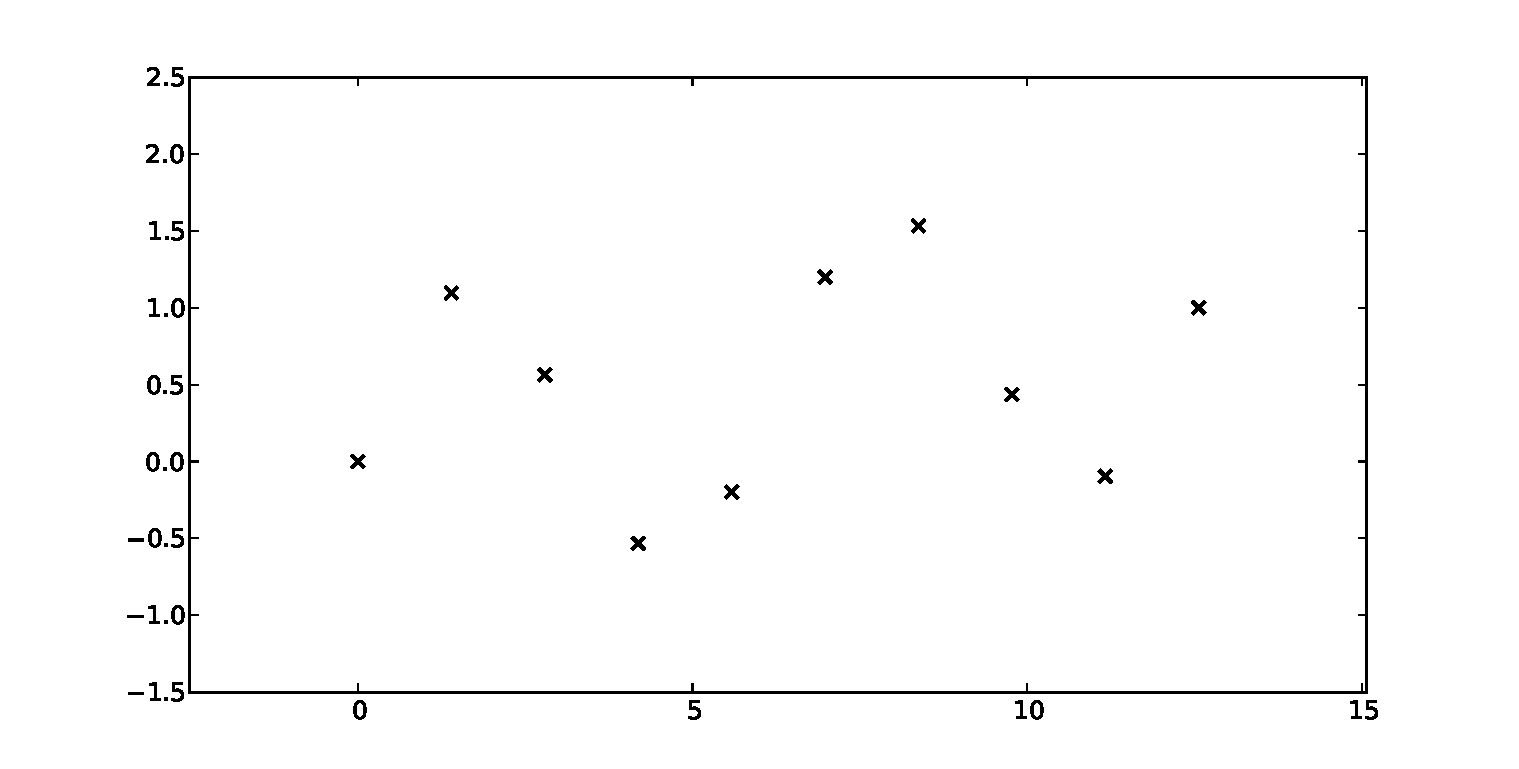
\includegraphics[height=4.5cm]{figures/Fig2-f}
\end{center}
\vspace{.3cm}
\end{block}
 Can we extract the periodic part of a signal ?\\
\end{frame}

%%%%%%%%%%%%%%%%%%%%%%%%%%%%%%%%%%%%%%%%%%%%%%%%%%%%%%
\begin{frame}{}
Let $Z$ be a GP and $B(t) = ( \sin(t), \cos(t), \dots, \sin(nt), cos(nt))^t$ be the fourier basis. We consider the projection of $Z$ onto the basis:
\small
$$Z_p(t) = \frac{ \PSi{Z,\sin}{} }{ \PSi{\sin,\sin}{} } \sin(t) +
\frac{ \PSi{Z,\cos}{} }{ \PSi{\cos,\cos}{} } \cos(t) +
\dots + 
\frac{ \PSi{Z,\cos(n.)}{} }{ \PSi{\cos(n.),\cos(n.)}{} } \cos(nt) $$
\normalsize
 This give a decomposition of the GP:
$$Z = Z_p + \underbrace{Z - Z_p}_{Z_a}.$$
By considering the appropriate inner product, we can ensure that $Z_p$ and $Z_a$ are independant. 
\vspace{0.2cm}
\begin{block}{Property}
 The reproducing kernel of $Z_p$ is 
 \begin{equation*}
  k_p(x,y) = B(x)^t G^{-1} B(y)
 \end{equation*}
 where $G$ is the Gram matrix $G$ associated to $B$.
\end{block}
\end{frame}

%%%%%%%%%%%%%%%%%%%%%%%%%%%%%%%%%%%%%%%%%%%%%%%%%%%%%%
\begin{frame}{}
We can deduce the following decomposition of the kernel:
 \small
 \begin{equation*}
  k(x,y) = k_p(x,y) + \underbrace{k(x,y) - k_p(x,y)}_{k_a(x,y)}
 \end{equation*}
\begin{block}{Property: Decomposition of the model}
 The decomposition of the kernel gives directly
 \small
 \begin{equation*}
 \begin{split}
  m(t) & = (k_p(t) + k_a(t))^t (K_p+K_a)^{-1} F \\
  &  = \underbrace{k_p(t)^t (K_p+K_a)^{-1} F}_{\text{periodic sub-model }m_p} + \underbrace{k_a(t)^t (K_p+K_a)^{-1} F}_{\text{aperiodic sub-model }m_a}
 \end{split}
 \end{equation*}
 \normalsize
and we can associate a prediction variance to the sub-models:
\small
\begin{equation*}
\begin{split}
 v_p(t) & = k_p(t,t) - k_p(t)^t (K_p+K_a)^{-1} k_p(t) \\
 v_a(t) & = k_a(t,t) - k_a(t)^t (K_p+K_a)^{-1} k_a(t)
\end{split}
\end{equation*}
\end{block}
\end{frame}

%%%%%%%%%%%%%%%%%%%%%%%%%%%%%%%%%%%%%%%%%%%%%%%%%%%%%%
\begin{frame}{}
\begin{example}
For the observations shown previously we obtain:
\begin{center}
 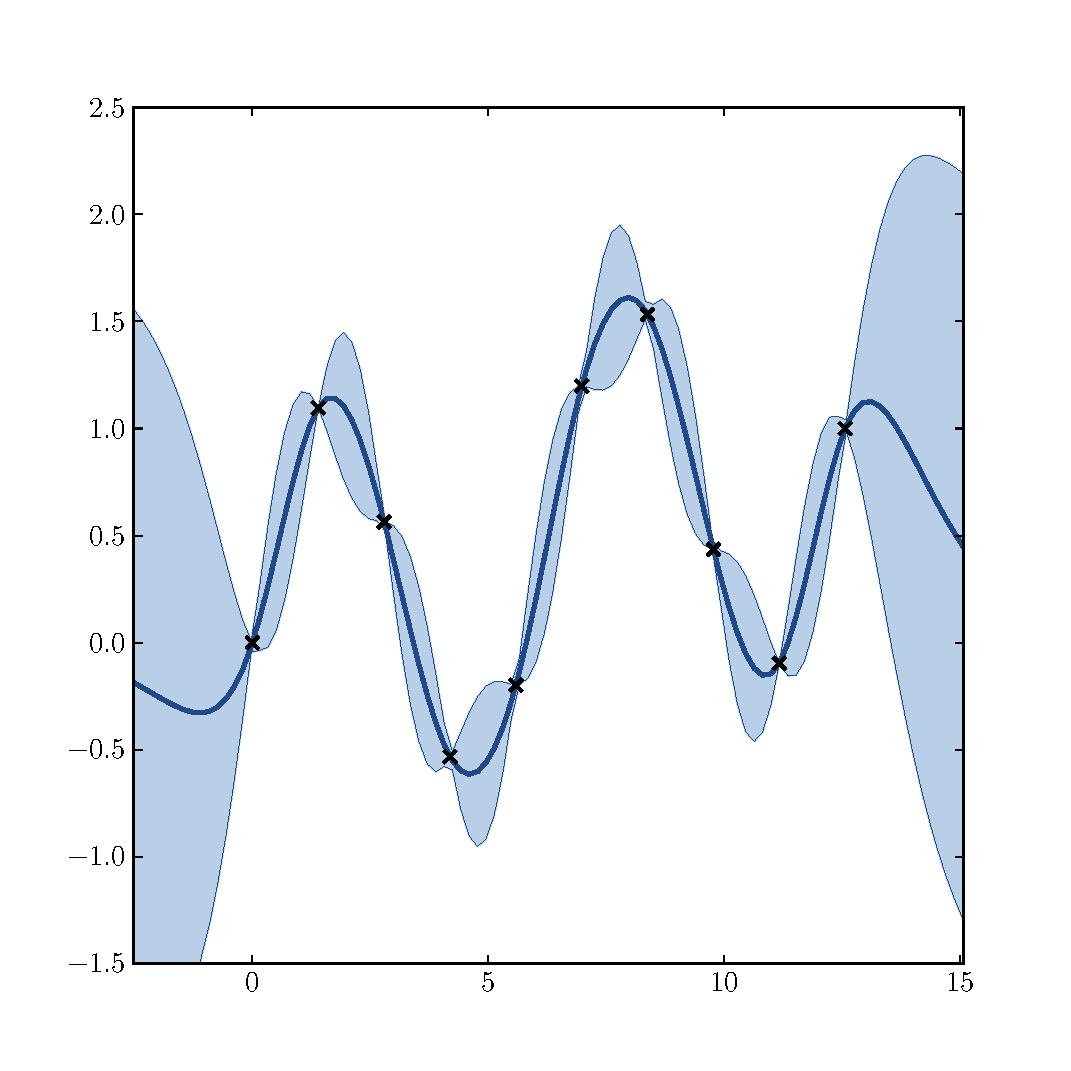
\includegraphics[height=4cm]{figures/Fig2-m} 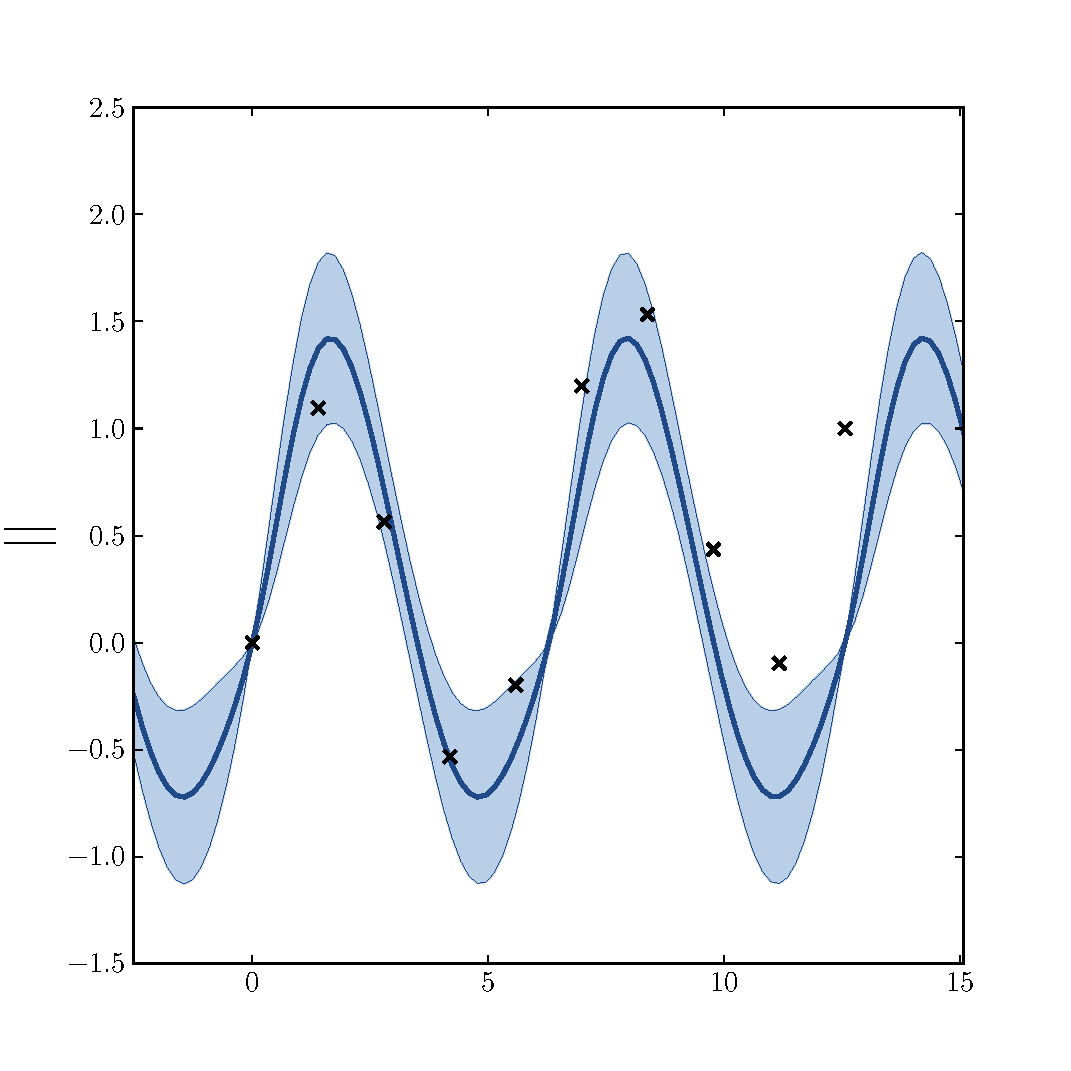
\includegraphics[height=4cm]{figures/Fig2-mp} 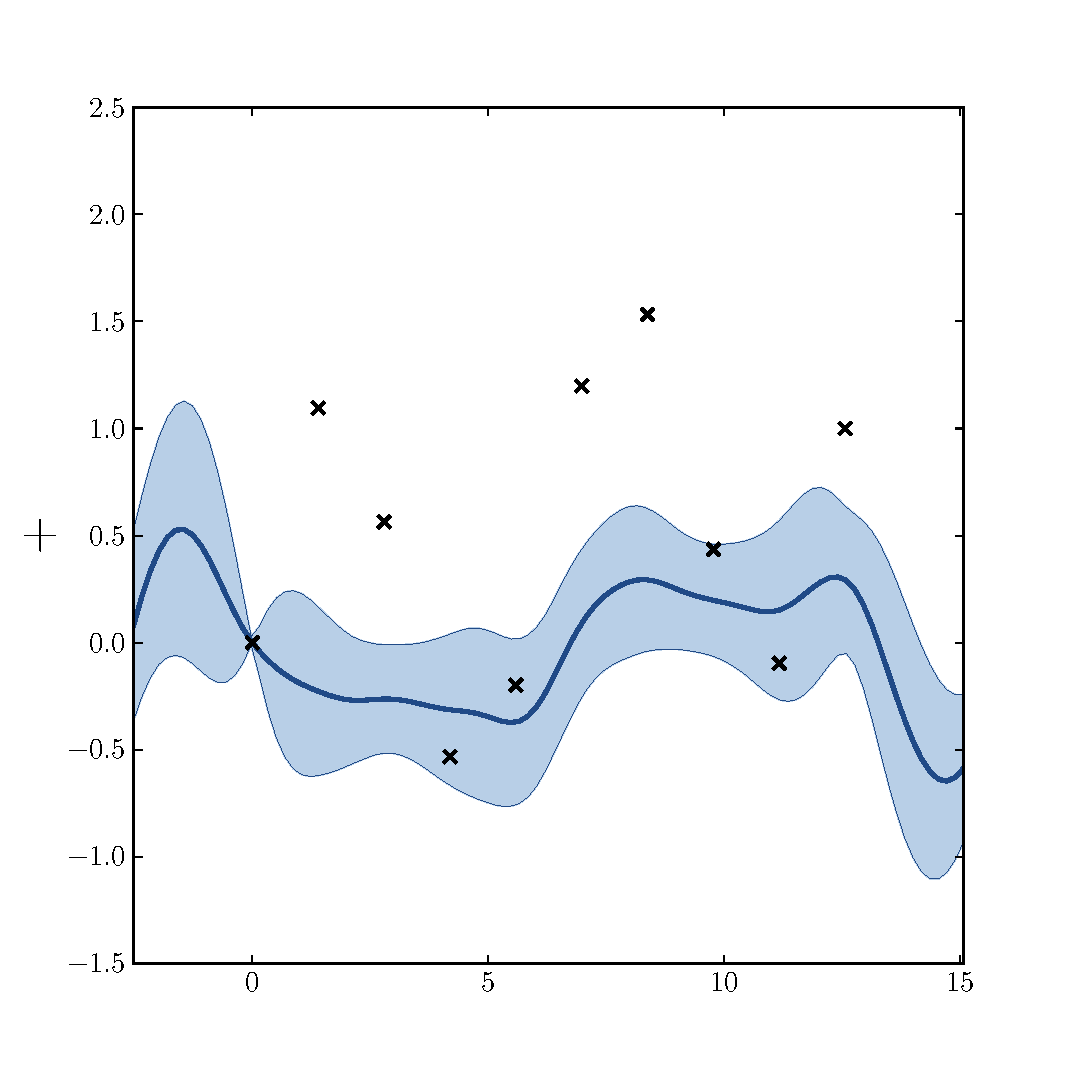
\includegraphics[height=4cm]{figures/Fig2-ma}
\end{center}
\end{example}
Can we can do better?\\ 
\end{frame}

%%%%%%%%%%%%%%%%%%%%%%%%%%%%%%%%%%%%%%%%%%%%%%%%%%%%%%
\begin{frame}{}
\begin{block}{}
Previously, the kernels were parameterized by 2 variables: 
\begin{equation*}
 k(x,y,\sigma^2, \theta)
\end{equation*}
but writing $k$ as a sum allows to tune independently the parameters of the sub-kernels.
\end{block}
Let $k^*$ be defined as
\begin{equation*}
 k^*(x,y,\sigma^2_p,\sigma^2_a, \theta_p, \theta_a) = k_p(x,y,\sigma^2_p, \theta_p) + k_a(x,y,\sigma^2_a, \theta_a)
\end{equation*}
Furthermore, we include a $5^{th}$ parameter in $k^*$ accounting for the period by changing the Fourier basis:
\begin{equation*}
 B_\omega(t) = (\sin(\omega t), \cos(\omega t), \dots, \sin(n \omega t), cos(n \omega t))^t
\end{equation*}
\end{frame}

%%%%%%%%%%%%%%%%%%%%%%%%%%%%%%%%%%%%%%%%%%%%%%%%%%%%%%
\begin{frame}{}
If we optimize the 5 parameters of $k^*$ with maximum likelihood estimation we obtain: 
\begin{center}
 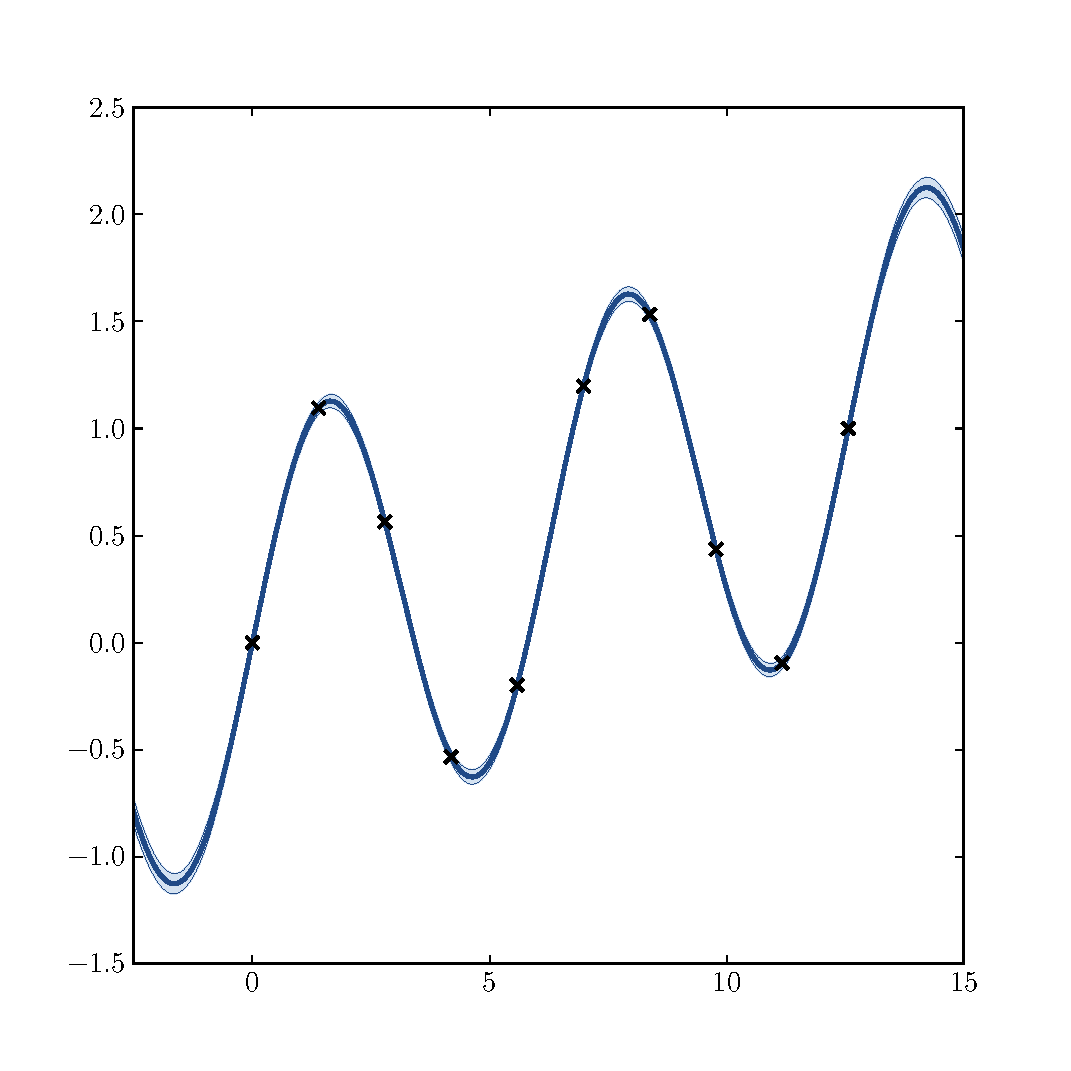
\includegraphics[height=4cm]{figures/Fig2-m-estim} 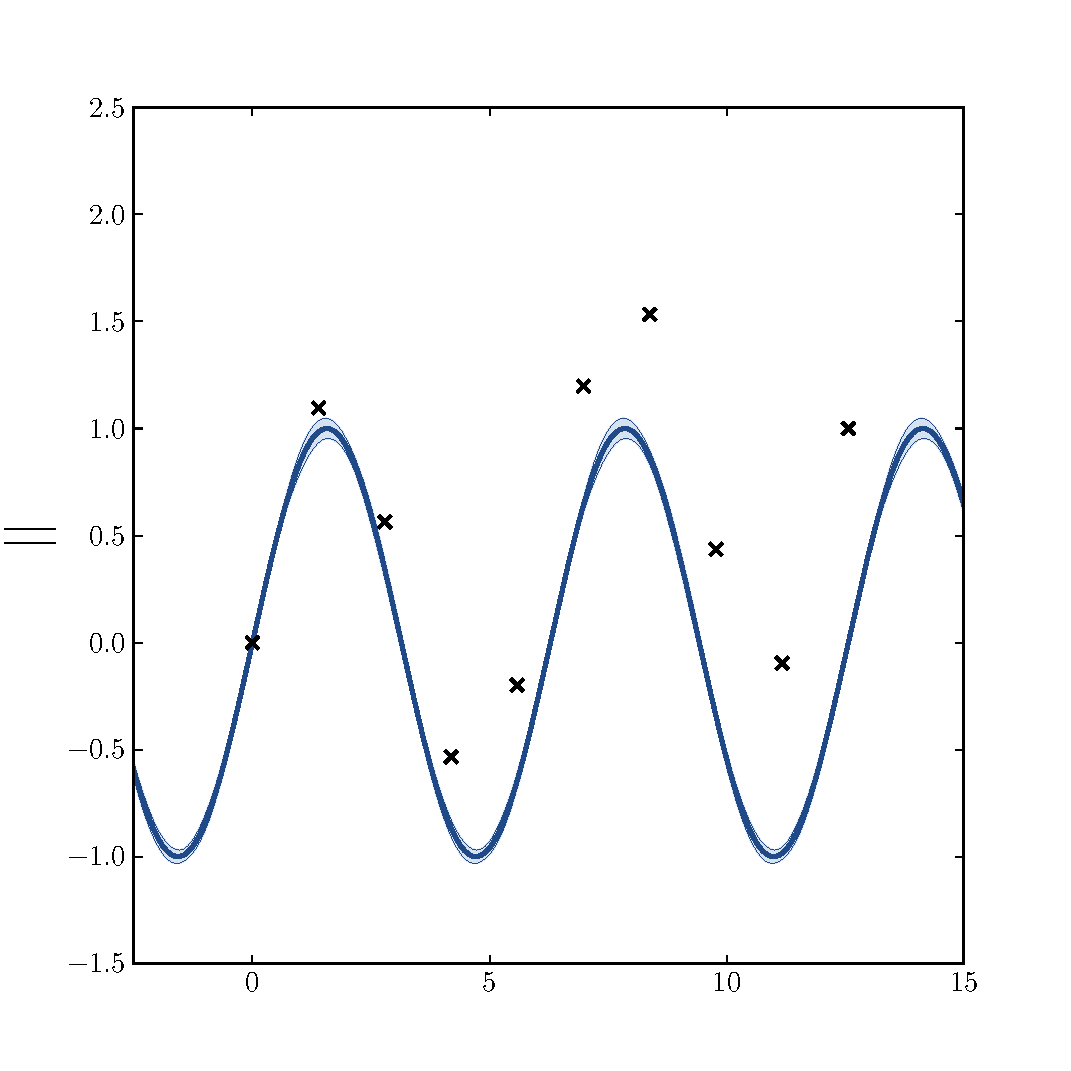
\includegraphics[height=4cm]{figures/Fig2-mp-estim-top} 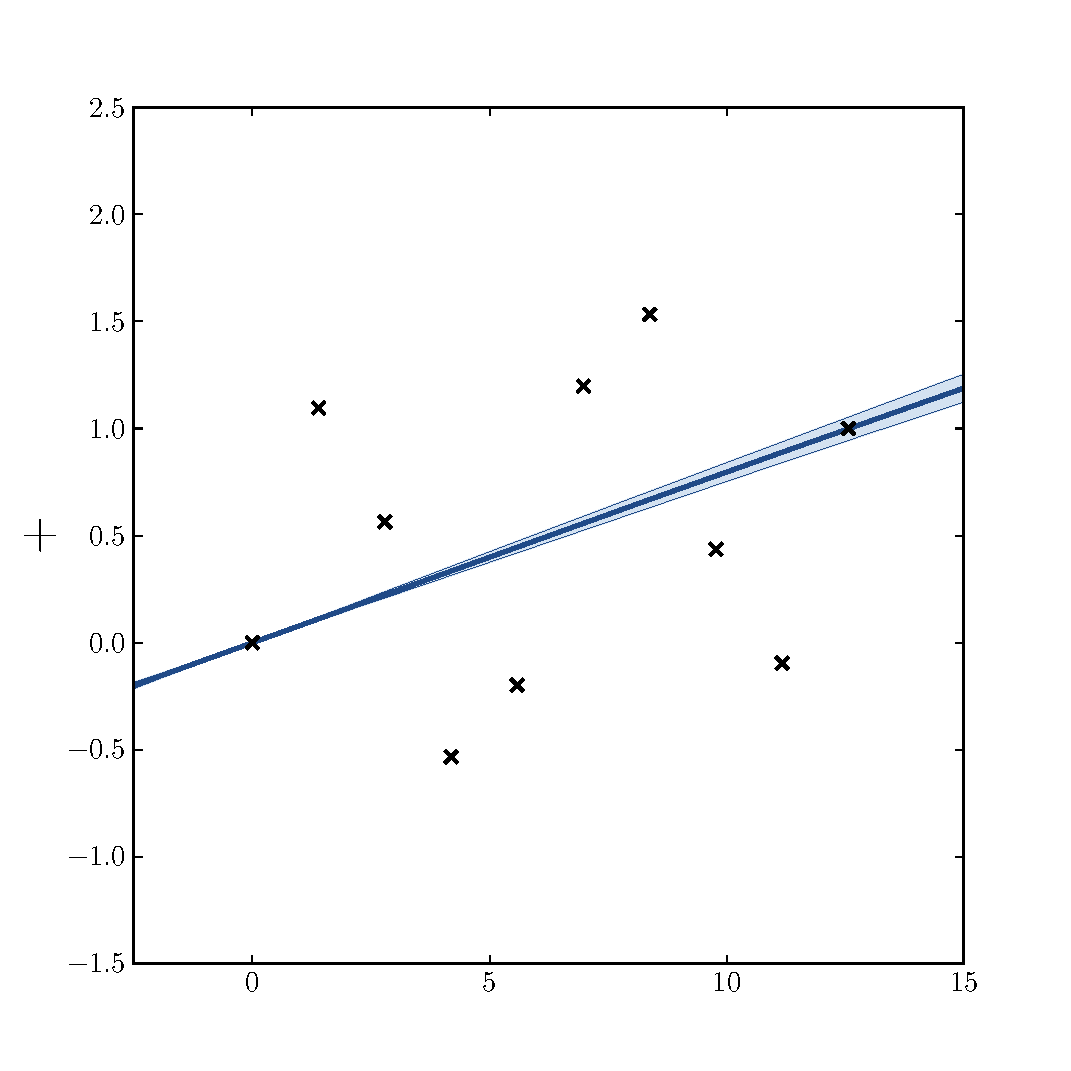
\includegraphics[height=4cm]{figures/Fig2-ma-estim-top}
\end{center}
\end{frame}


%%%%%%%%%%%%%%%%%%%%%%%%%%%%%%%%%%%%%%%%%%%%%%%%%%%%%%
\begin{frame}{}
\vspace{0.5cm}
We used data from Edward 2006, based on \textit{arabidopsis}.
\begin{columns}[c]
\column{5cm}
The dimension of the data is:
\begin{itemize}
 \item 22810 genes
 \item 13 time points
\end{itemize}
\column{5cm}
\begin{center}
 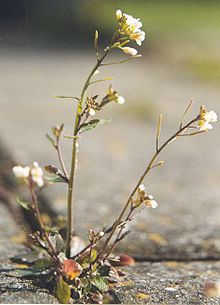
\includegraphics[height=4cm]{figures/Arabidopsis}
\end{center}
\end{columns}
\begin{block}{}
 Edward 2006 gives a list of the 3504 most periodically expressed genes. The comparison with our approach gives:
 \begin{itemize}
 \item 21767 genes with the same label (2461 per. and 19306 non-per.)
 \item 1043 genes with different labels
\end{itemize}
\end{block}
\end{frame}

%%%%%%%%%%%%%%%%%%%%%%%%%%%%%%%%%%%%%%%%%%%%%%%%%%%%%%
\begin{frame}{}
Let's look at genes with different labels:
\begin{center}
 \begin{tabular}{ccc}
  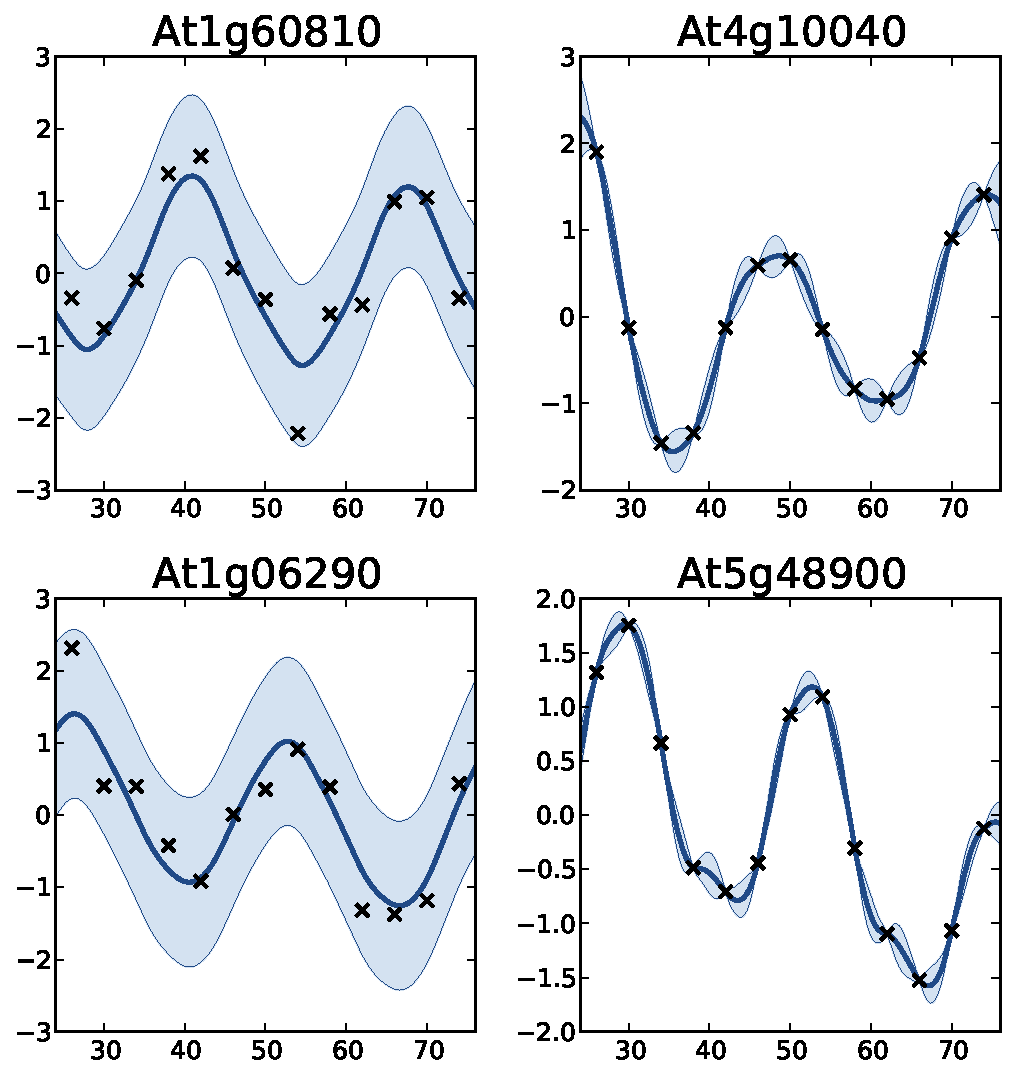
\includegraphics[height=5cm]{figures/per_Ed_Only.pdf} & \qquad &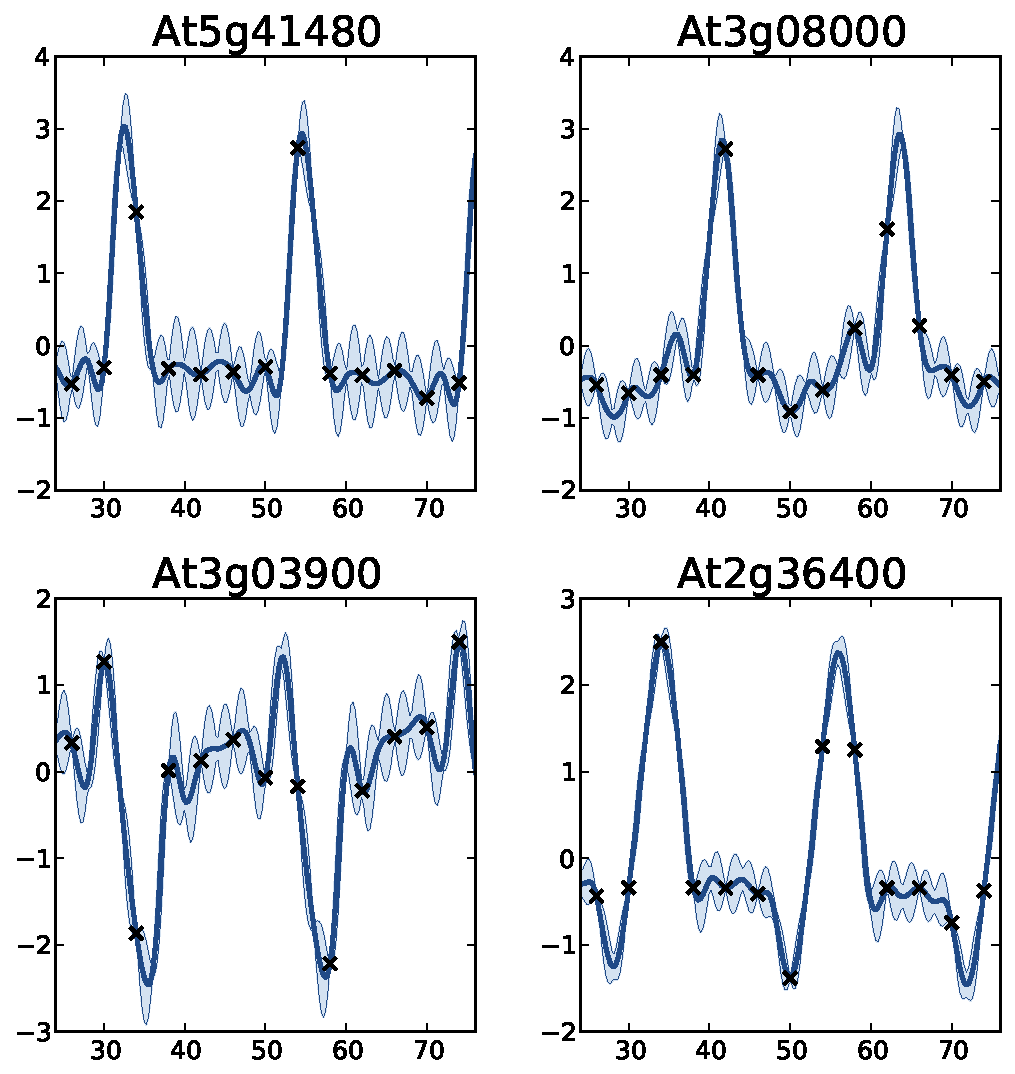
\includegraphics[height=5cm]{figures/per_RKHS_Only.pdf} \\
  {\small periodic for Edward} & & {\small periodic for our approach}
 \end{tabular}
\end{center}
\end{frame}

%%%%%%%%%%%%%%%%%%%%%%%%%%%%%%%%%%%%%%%%%%%%%%%%%%%%%%%%%%%%%%%%%%%%%%%%%%%%%
%%%%%%%%%%%%%%%%%%%%%%%%%%%%%%%%%%%%%%%%%%%%%%%%%%%%%%%%%%%%%%%%%%%%%%%%%%%%%
\section[GP classification]{GP models for classification}
\subsection{}

%%%%%%%%%%%%%%%%%%%%%%%%%%%%%%%%%%%%%%%%%%%%%%%%%%%%%%
\begin{frame}{}
Until now, we have focused on GP \textbf{Regression}: we were using GPs to predict a continuous output given some input values.\\
\vspace{5mm} 
Gaussian process models are also useful for \textbf{classification} problems:
\begin{center}
 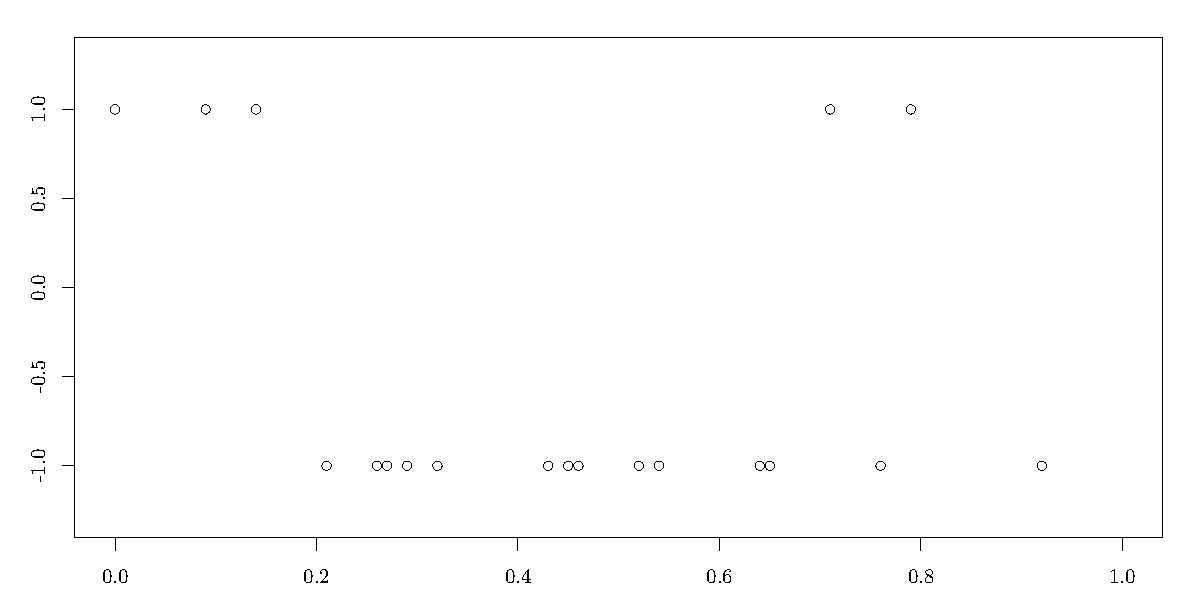
\includegraphics[height=5cm]{figures/R/classif_data.pdf}
\end{center}
\end{frame}

%%%%%%%%%%%%%%%%%%%%%%%%%%%%%%%%%%%%%%%%%%%%%%%%%%%%%%
\begin{frame}{}
We consider the following probabilistic model for the data
\begin{enumerate}
 	\item Let $Y$ be a Gaussian process over $\mathds{R}$.
 	\item Let $\Phi$ be a sigmoid transformation such as
 	$$ \Phi(y) = \frac{1}{1+e^{-y}} \text{\qquad \textbf{or} \qquad $\Phi$ is the Gaussian cdf.}$$ 
 	\item We denote by $Z$ the image of $Y$ by $\Phi$: $Z(x) = \Phi(Y(x))$.
 	\item The observation $F_i \in \{-1,\ 1\}$ at input $X_i$ is given by a Bernouilli sample with parameter $Z(X_i)$.
 \end{enumerate}
\end{frame}

%%%%%%%%%%%%%%%%%%%%%%%%%%%%%%%%%%%%%%%%%%%%%%%%%%%%%%
\begin{frame}{}
Same thing with images\\
% \begin{center}
 \begin{tabular}{ccc}
  GP $Y(x)$ & $Z(x)=\Phi(Y(x))$ & $F_i \sim \mathcal{B}(Z(X_i))$ iid \\
  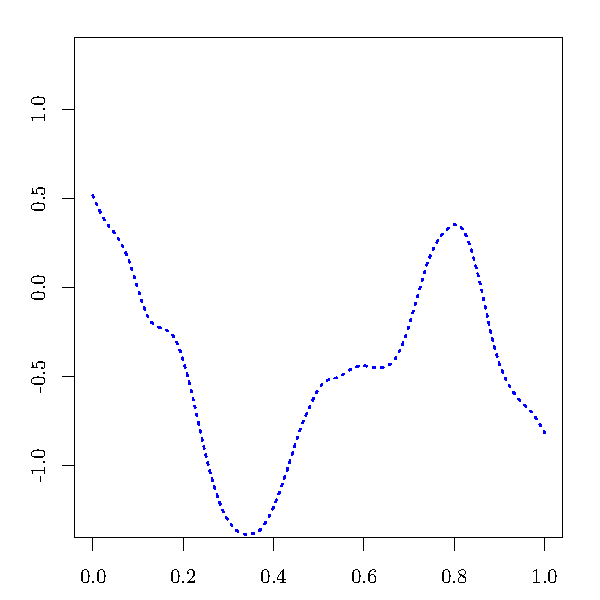
\includegraphics[height=3.5cm]{figures/R/classif_GP.pdf} & 
  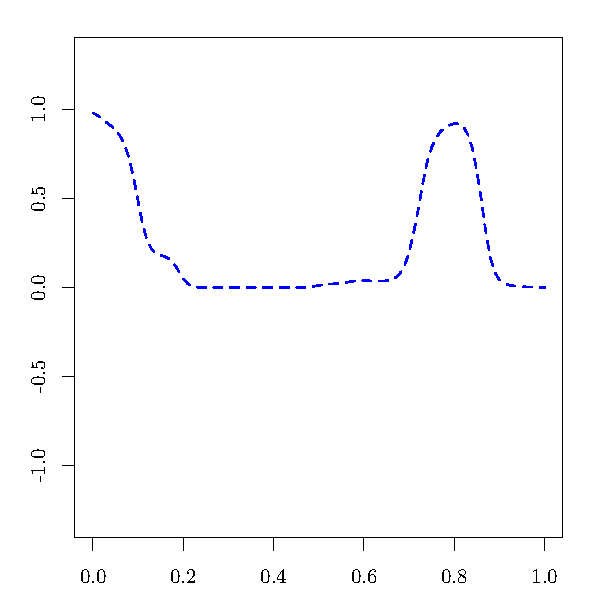
\includegraphics[height=3.5cm]{figures/R/classif_phiGP.pdf} &
  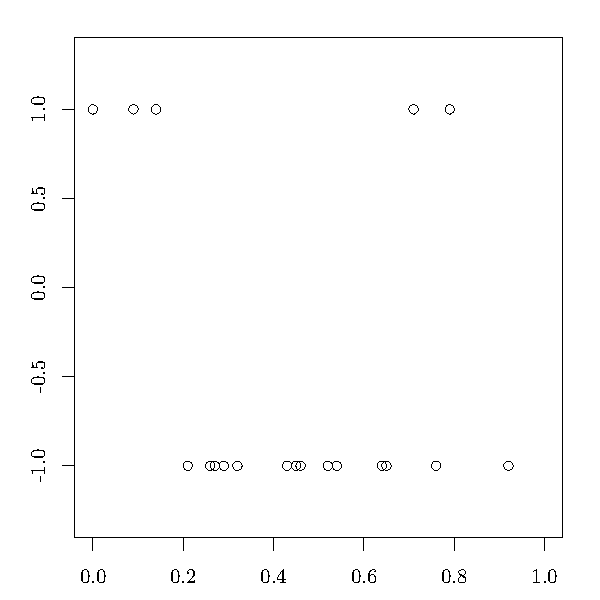
\includegraphics[height=3.5cm]{figures/R/classif_datasmall.pdf} \\
 \end{tabular}
% \end{center}
\end{frame}

%%%%%%%%%%%%%%%%%%%%%%%%%%%%%%%%%%%%%%%%%%%%%%%%%%%%%%
\begin{frame}{}
In order to make predictions, we need to compute the conditional distribution of $Y$ (or $Z$) given the observed data: $Y$ and $Z$ are called latent variables because we never have observations of them.\\
\vspace{5mm}
\begin{exampleblock}{Exercise}
	\begin{enumerate}
		\item Is the vector $(Y,F)$ a Gaussian vector?
		\item What can you say about $P(F_i|Y(X_i))$? Deduce the probability of $P((F_1,F_2)|Y(X_1),Y(X_2))$. 
		\item Use Bayes rule to re-write the conditional pdf of $(Y(X_1),Y(X_2))$ given the observations $(F_1,F_2)$.
		\item Give a graphical representation of this conditional distribution. 
	\end{enumerate}
\end{exampleblock}
\end{frame}

%%%%%%%%%%%%%%%%%%%%%%%%%%%%%%%%%%%%%%%%%%%%%%%%%%%%%%
\begin{frame}{}
Examples of posteriors
\begin{center}
 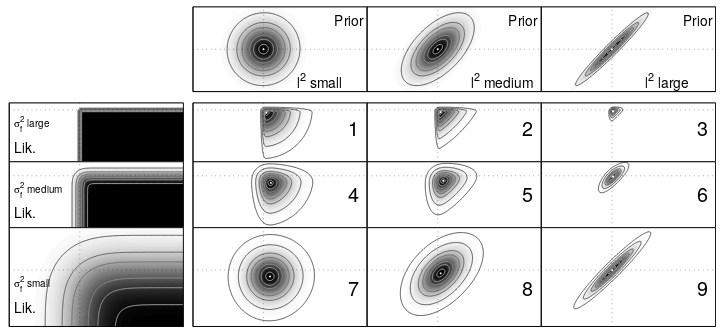
\includegraphics[height=5cm]{figures/classif_post}
\end{center}
\begin{flushright}
{\small \emph{source:} Nickisch and Rasmussen, JMLR 2008.}
\end{flushright}
\end{frame}

%%%%%%%%%%%%%%%%%%%%%%%%%%%%%%%%%%%%%%%%%%%%%%%%%%%%%%
\begin{frame}{}
The conditional distribution of $Y|F$ is not Gaussian... In practice it is possible to:
\begin{itemize}
	\item Use the mode of the distribution.
	\item Sample from the distribution using MCMC.
	\item Make a Gaussian approximation of this non Gaussian distribution:
	\begin{itemize}
		\item Laplace method
		\item Variational inference
		\item ...
	\end{itemize}
\end{itemize}
Once the distribution of $Y(X)|F$ has been approximated, we can deduce the distribution of $Y(x)|F$. It is then possible to obtain predictions for the labels of future observations at $x$.
\end{frame}


%%%%%%%%%%%%%%%%%%%%%%%%%%%%%%%%%%%%%%%%%%%%%%%%%%%%%%
\begin{frame}{}
As for GPR, GP classification models are straightforward to generalize in higher dimension
\begin{center}
 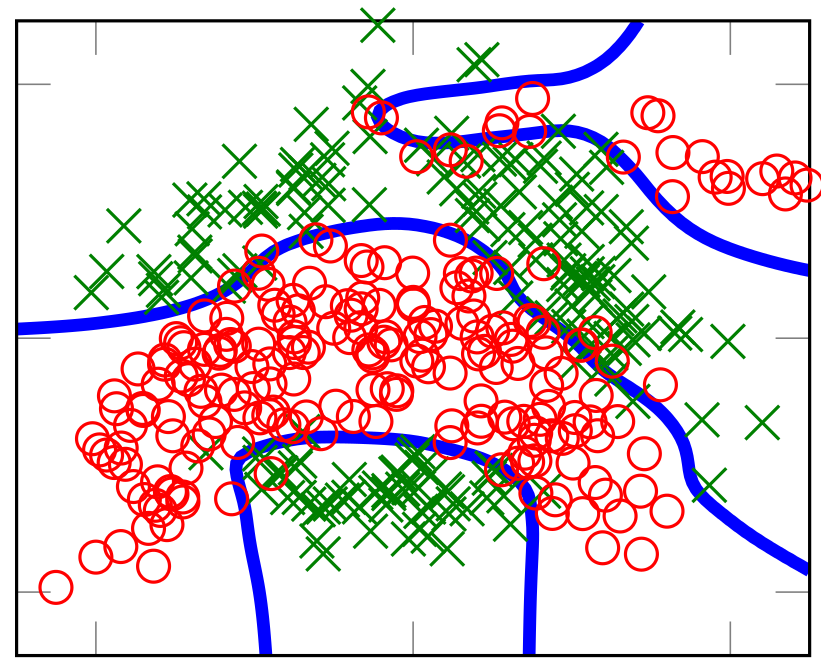
\includegraphics[height=5cm]{figures/classif_2d}
\end{center}
\begin{flushright}
{\small \emph{source:} Hensman, Durrande and Solin, arXiv 2016.}
\end{flushright}
\end{frame}


%%%%%%%%%%%%%%%%%%%%%%%%%%%%%%%%%%%%%%%%%%%%%%%%%%%%%%%%%%%%%%%%%%%%%%%%%%%%%
%%%%%%%%%%%%%%%%%%%%%%%%%%%%%%%%%%%%%%%%%%%%%%%%%%%%%%%%%%%%%%%%%%%%%%%%%%%%%
\section{Conclusion}
\subsection{}

%%%%%%%%%%%%%%%%%%%%%%%%%%%%%%%%%%%%%%%%%%%%%%%%%%%%%%
\begin{frame}{}
\begin{block}{We have seen that}
\begin{itemize}
 \item Gaussian processes are a great tool for modeling
 \begin{itemize}
 	\item Regression and classification
 \end{itemize}
 \item Kernels can (and should) be tailored to the problem at hand
 \item It is possible to include in models more that function values 
\end{itemize}
\end{block}
\vspace{0.2cm}
\begin{block}{What we have not seen...}
\begin{itemize}
 \item Unsupervised models: non-linear generalization of PCA
 \item How to deal with a (very) large number of observations
 \item links with the RKHS theory
 \item ...
\end{itemize}
\end{block}
\vspace{0.2cm}
Gaussian process models are of \textbf{particular interest in industry}, and they are also an \textbf{active research topic}...
\end{frame}



\end{document}
%%%%%%%%%%%%%%%%%%%%%%%%%%%%%%%%%%%%%%%%%%%%%%%%%%%%%%%%%%%%%%%%%%%%%%%%%%%%%%%
%%%%%%%%%%%%%%%%%%%%%%%%%%%%%%%%%%%%%%%%%%%%%%%%%%%%%%%%%%%%%%%%%%%%%%%%%%%%%%%
%%%%%%%%%%%%%%%%%%%%%%%%%%%%%%%%%%%%%%%%%%%%%%%%%%%%%%%%%%%%%%%%%%%%%%%%%%%%%%%
%%%%%%%%%%%%%%%%%%%%%%%%%%%%%%%%%%%%%%%%%%%%%%%%%%%%%%%%%%%%%%%%%%%%%%%%%%%%%%%



\structure{}

\begin{center}
  \begin{tabular}{|c|cc|}

  \end{tabular}
\end{center}

###
%%%%%%%%%%%%%%%%%%%%%%%%%%%%%%%%%%%%%%%%%%%%%%%%%%%%%%
\begin{frame}{}

\end{frame}

###
\begin{block}{}

\end{block}

###
\begin{center}
\includegraphics[height=5cm]{figures/}
\end{center}

###
\begin{columns}[c]
\column{5cm}

\column{5cm}

\end{columns}
